% Template for PLoS
% Version 3.3 June 2016
%
% % % % % % % % % % % % % % % % % % % % % %
%
% -- IMPORTANT NOTE
%
% This template contains comments intended 
% to minimize problems and delays during our production 
% process. Please follow the template instructions
% whenever possible.
%
% % % % % % % % % % % % % % % % % % % % % % % 
%
% Once your paper is accepted for publication, 
% PLEASE REMOVE ALL TRACKED CHANGES in this file 
% and leave only the final text of your manuscript. 
% PLOS recommends the use of latexdiff to track changes during review, as this will help to maintain a clean tex file.
% Visit https://www.ctan.org/pkg/latexdiff?lang=en for info or contact us at latex@plos.org.
%
%
% There are no restrictions on package use within the LaTeX files except that 
% no packages listed in the template may be deleted.
%
% Please do not include colors or graphics in the text.
%
% The manuscript LaTeX source should be contained within a single file (do not use \input, \externaldocument, or similar commands).
%
% % % % % % % % % % % % % % % % % % % % % % %
%
% -- FIGURES AND TABLES
%
% Please include tables/figure captions directly after the paragraph where they are first cited in the text.
%
% DO NOT INCLUDE GRAPHICS IN YOUR MANUSCRIPT
% - Figures should be uploaded separately from your manuscript file. 
% - Figures generated using LaTeX should be extracted and removed from the PDF before submission. 
% - Figures containing multiple panels/subfigures must be combined into one image file before submission.
% For figure citations, please use "Fig" instead of "Figure".
% See http://journals.plos.org/plosone/s/figures for PLOS figure guidelines.
%
% Tables should be cell-based and may not contain:
% - spacing/line breaks within cells to alter layout or alignment
% - do not nest tabular environments (no tabular environments within tabular environments)
% - no graphics or colored text (cell background color/shading OK)
% See http://journals.plos.org/plosone/s/tables for table guidelines.
%
% For tables that exceed the width of the text column, use the adjustwidth environment as illustrated in the example table in text below.
%
% % % % % % % % % % % % % % % % % % % % % % % %
%
% -- EQUATIONS, MATH SYMBOLS, SUBSCRIPTS, AND SUPERSCRIPTS
%
% IMPORTANT
% Below are a few tips to help format your equations and other special characters according to our specifications. For more tips to help reduce the possibility of formatting errors during conversion, please see our LaTeX guidelines at http://journals.plos.org/plosone/s/latex
%
% For inline equations, please be sure to include all portions of an equation in the math environment.  For example, x$^2$ is incorrect; this should be formatted as $x^2$ (or $\mathrm{x}^2$ if the romanized font is desired).
%
% Do not include text that is not math in the math environment. For example, CO2 should be written as CO\textsubscript{2} instead of CO$_2$.
%
% Please add line breaks to long display equations when possible in order to fit size of the column. 
%
% For inline equations, please do not include punctuation (commas, etc) within the math environment unless this is part of the equation.
%
% When adding superscript or subscripts outside of brackets/braces, please group using {}.  For example, change "[U(D,E,\gamma)]^2" to "{[U(D,E,\gamma)]}^2". 
%
% Do not use \cal for caligraphic font.  Instead, use \mathcal{}
%
% % % % % % % % % % % % % % % % % % % % % % % % 
%
% Please contact latex@plos.org with any questions.
%
% % % % % % % % % % % % % % % % % % % % % % % %

\documentclass[10pt,letterpaper]{article}
\usepackage[top=0.85in,left=2.75in,footskip=0.75in]{geometry}

% amsmath and amssymb packages, useful for mathematical formulas and symbols
\usepackage{amsmath,amssymb}

% Use adjustwidth environment to exceed column width (see example table in text)
\usepackage{changepage}

% Use Unicode characters when possible
\usepackage[utf8x]{inputenc}

% textcomp package and marvosym package for additional characters
\usepackage{textcomp,marvosym}

% cite package, to clean up citations in the main text. Do not remove.
\usepackage{cite}

% makes the \textsubscript work on my older version of latex
\usepackage{fixltx2e}

% Use nameref to cite supporting information files (see Supporting Information section for more info)
\usepackage{nameref,hyperref}

% line numbers
\usepackage[right]{lineno}

% ligatures disabled
\usepackage{microtype}
\DisableLigatures[f]{encoding = *, family = * }

% color can be used to apply background shading to table cells only
\usepackage[table]{xcolor}
\usepackage{multirow} %connecting columns in tables
\usepackage{multicol}
\usepackage{longtable}

% array package and thick rules for tables
\usepackage{array}

% create "+" rule type for thick vertical lines
\newcolumntype{+}{!{\vrule width 2pt}}

% create \thickcline for thick horizontal lines of variable length
\newlength\savedwidth
\newcommand\thickcline[1]{%
  \noalign{\global\savedwidth\arrayrulewidth\global\arrayrulewidth 2pt}%
  \cline{#1}%
  \noalign{\vskip\arrayrulewidth}%
  \noalign{\global\arrayrulewidth\savedwidth}%
}

% \thickhline command for thick horizontal lines that span the table
\newcommand\thickhline{\noalign{\global\savedwidth\arrayrulewidth\global\arrayrulewidth 2pt}%
\hline
\noalign{\global\arrayrulewidth\savedwidth}}


% Remove comment for double spacing
%\usepackage{setspace} 
%\doublespacing

% Text layout
\raggedright
\setlength{\parindent}{0.5cm}
\textwidth 5.25in 
\textheight 8.75in

% Bold the 'Figure #' in the caption and separate it from the title/caption with a period
% Captions will be left justified
\usepackage[aboveskip=1pt,labelfont=bf,labelsep=period,justification=raggedright,singlelinecheck=off]{caption}
\renewcommand{\figurename}{Fig}

% Use the PLoS provided BiBTeX style
\bibliographystyle{plos2015}

% Remove brackets from numbering in List of References
\makeatletter
\renewcommand{\@biblabel}[1]{\quad#1.}
\makeatother

% Leave date blank
\date{}

% Header and Footer with logo
\usepackage{lastpage,fancyhdr,graphicx}
\usepackage{epstopdf}
\pagestyle{myheadings}
\pagestyle{fancy}
\fancyhf{}
\setlength{\headheight}{27.023pt}
\lhead{\includegraphics[width=2.0in]{PLOS-submission.eps}}
\rfoot{\thepage/\pageref{LastPage}}
\renewcommand{\footrule}{\hrule height 2pt \vspace{2mm}}
\fancyheadoffset[L]{2.25in}
\fancyfootoffset[L]{2.25in}
\lfoot{\sf PLOS}

%% Include all macros below

\newcommand{\lorem}{{\bf LOREM}}
\newcommand{\ipsum}{{\bf IPSUM}}

%% END MACROS SECTION


\begin{document}
\vspace*{0.2in}

% Title must be 250 characters or less.
\begin{flushleft}
{\Large
\textbf\newline{Eco-evolutionary Dynamics on the Invasion Front Drives the Co-existence of Target Site and Quantitative Resistance} % Please use "title case" (capitalize all terms in the title except conjunctions, prepositions, and articles).
}
\newline
% Insert author names, affiliations and corresponding author email (do not include titles, positions, or degrees).
\\
Shaun Coutts\textsuperscript{1*},
Rob Freckelton\textsuperscript{1},
Helen Hicks\textsuperscript{1},
Paul Neve\textsuperscript{2},
Dylan Childs\textsuperscript{1},
\\
\bigskip
\textbf{1} Animal and Plant Sciences, University of Sheffield, Sheffield, UK
\\
\textbf{2} Affiliation Dept/Program/Center, Institution Name, City, State, Country
\\
\bigskip

% Insert additional author notes using the symbols described below. Insert symbol callouts after author names as necessary.
% 
% Remove or comment out the author notes below if they aren't used.
%
% Primary Equal Contribution Note
%\Yinyang These authors contributed equally to this work.

% Additional Equal Contribution Note
% Also use this double-dagger symbol for special authorship notes, such as senior authorship.
%\ddag These authors also contributed equally to this work.

% Current address notes
%\textcurrency Current Address: Dept/Program/Center, Institution Name, City, State, Country % change symbol to "\textcurrency a" if more than one current address note
% \textcurrency b Insert second current address 
% \textcurrency c Insert third current address

% Deceased author note
%\dag Deceased

% Group/Consortium Author Note
%\textpilcrow Membership list can be found in the Acknowledgments section.

% Use the asterisk to denote corresponding authorship and provide email address in note below.
* shaun.coutts@gmail.com

\end{flushleft}
% Please keep the abstract below 300 words
\section*{Abstract}
Lorem ipsum dolor sit amet, consectetur adipiscing elit. Curabitur eget porta erat. Morbi consectetur est vel gravida pretium. Suspendisse ut dui eu ante cursus gravida non sed sem. Nullam sapien tellus, commodo id velit id, eleifend volutpat quam. Phasellus mauris velit, dapibus finibus elementum vel, pulvinar non tellus. Nunc pellentesque pretium diam, quis maximus dolor faucibus id. Nunc convallis sodales ante, ut ullamcorper est egestas vitae. Nam sit amet enim ultrices, ultrices elit pulvinar, volutpat risus.


% Please keep the Author Summary between 150 and 200 words
\section*{Author Summary}

\linenumbers

% Use "Eq" instead of "Equation" for equation citations.
\section*{Introduction}
There is currently a global resistance crisis \cite{Serv2013, Ross2014} and important antibiotics, pesticides and herbicides are losing their efficacy \cite{Palu2001}. Together, these chemical tools are a crucial part of the worlds food productions system \cite{Duke2012}, and are used worldwide to control life threatening bacterial infections and diseases spread by insects \cite{Nkya2013}, however, evolving resistance threatens their continued use \cite{Barb2011, Nkya2013}. Economic and regulatory conditions mean that bringing new, safe, effective, compounds to market is time consuming and expensive \cite{Duke2012}. In addition, the useful life of new chemical tools can be as short as three years if their use is not well managed \cite{Palu2001, Duke2012}. To address this crisis and reduce its impact we need to understand where and when resistance will evolve, and under what conditions. 

Until recently, target site resistance, conferred by a single gene of large effect, has formed the basis of our understanding of resistance, and the evolution of target site resistance is well understood \cite{Neve2007}. However, evolutionary biologists have recognized a continuum in the genetic architecture underlying any given trait since the early 20th century (genetic architecture \textit{sensu} \cite{Deba2015}, the number and effect size of loci contributing to a trait). At one extreme traits are controlled by a single loci of large effect (as in the case of target site resistance), and at the other polygenic, quantitative traits, are controlled by smaller additive effects of many genes \cite{Land1989, Mack2009, Rajo2013}. There is growing evidence that within the same population, resistance can be conferred by genetic architectures at both extremes \cite{Donn2009, Bing2011, Hend2013, Oake2013, Bauc2016}. The implications for the evolution of these multi-architecture traits remains largely unexplored, and how multi-architecture traits interact over space is not well understood (see \cite{Deba2015}, \cite{Yeam2015} for exceptions). Such an understanding will be crucial to predict how target site and quantitative resistance interact to drive the evolution and spread of resistant genotypes through populations.

Target site resistance typically confers very high levels of resistance, and incurs very few life history costs (i.e. reductions in survival, growth and/or fecundity). Quantitative resistance is usually achieved by metabolizing the poison, or transporting the poison away from its binding site \cite{Bauc2016} and tends to confer lower levels of resistance and incur life history costs \cite{Bauc2016}. It is currently unknown how these two genetic architectures interact in the evolution of resistance. Naively, we might expect the architecture that evolves first to reduce the selective pressure for the second architecture, and so slow its evolution. However, there is some evidence from misquote control programs that low levels of resistance conferred via an inefficient quantitative pathway can increase the rate of evolution for a much less costly target site mutation that confers high levels of resistance \cite{Vera2015}.

In many cases, herbicide resistance does not evolve in all the places where the trait is expressed; instead, resistance is often imported via pollen or seeds (ref). We expect this phenomena to affect target site resistance and quantitative resistance differently. Target site resistance can first enter a population in two ways: either it can be imported, which will often result in a small number of initial target site resistance individuals, perhaps just a single seed; or it can arise \textit{in situ} through mutation at a single loci. Both long distance dispersal and mutations are rare events, and so it is expected that initially target site resistance will be a rare and binary trait (either an individual is resistant or not). This will result in very little initial standing variation in target site resistance for selection to act upon, leading to a slow spread through the population once introduced. Conversely, Quantitative resistance is thought to co-opt existing stress tolerance strategies (ref), as a result all individuals in a population will have some level of quantitative resistance, although that level might be very low. Further, since quantitative resistance is regulated by multiple genes with additive effects, that quantitative resistance will be approximately normally distributed \cite{Land1989, Mack2009, Rajo2013}. This means that even naive populations that have never before been exposed to herbicide will have standing variation in quantitative resistance on which selection can act. These differences suggest that importation of resistance may be more important for target site resistance. Clumping of genotypes (due to dispersal limitation in seeds and pollen) could allow target site resistance to take hold more quickly, since individuals with rare genotypes (like initial target site resistant mutants) will be more likely to cross with other rare mutants if closely related individuals exist spatially close to each other (i.e. sibling-sibling crosses and parent-child crosses). However, once target site resistance is established, dispersal limitation will restrict its spread through the population. 

We develop one of the first spatially explicit, density dependent population models of the evolution of resistance as a complex, duel architecture trait. We apply this model to the economically important weed, \textit{Alopecurus myosuroides} (Huds.). Specifically, we test if quantitative resistance can slow the spread of target site resistance into a population, and if so under which range of costs for quantitative resistance. We also test how gene dispersal affects where and when both target site and quantitative resistance develop in the same population. 

\section*{Materials and Methods}
% For figure citations, please use "Fig" instead of "Figure".
\subsection*{model}
We model the invasion of a target site resistant genotype into a population of \textit{A. myosuroides} where quantitative resistance can also develop. \textit{A. myosuroides} is an annual, out-crossing grass. We use a flexible, discreet time, continuous space, modelling framework that can track the evolution of both continuous (quantitative resistance) and discreet (target site resistance) traits at the population level, called Integral Projection Models \cite{Elln2006}.     

We model a population of \textit{A. myosuroides} on a 1D landscape using a yearly time step, starting at the beginning of the growing season before any seeds have emerged from the seed bank. Once seeds emerge they are either exposed to herbicide or not, which affects their survival. Survival under herbicide is conferred by two types of resistance, quantitative and target site. Quantitative resistance is conferred trait $g$. All individuals have some value for $g$, but that value may be very small, and so phenotypically individuals are susceptible. We assume target site resistance is controlled by a single loci, with inheritance following simple two allele gene and random mating. We denote the resistant allele $R$ and the susceptible allele $r$. Those individuals that survive then flower and spread pollen. Finally, survivors disperse their seeds into the seed bank.  

All seeds in the seed bank at location $x$, time $t$, with target site genotype $G$ are distributed over metabolic resistance score $g$,
\begin{equation}\label{eq:seedbank_simp}
	b(g, G, x, t + 1) = b(g, G, x, t)(1 - \phi_e)\phi_b + f(g, G, h, x, t). 
\end{equation}
The first term in Eq. \ref{eq:seedbank_simp} is the distribution of surviving seeds in the seed bank of genotype $G$ at location $x$, where $\phi_e$ is the probability that a seed germinates and $\phi_b$ is the probability that a seed in the seed bank survives one year. The second term, $f(g, G, h, x, t)$, is the distribution of new seeds of genotype $G$ added to the population at location $x$. Note that $b(g, G, x, t)$ and $f(g, G, h, x, t)$ are distributions over metabolic resistance score $g$ and locations $x$. To get the total number of seeds for genotype $G$ these distributions have to be integrated over $g$ and $x$. Also note that we expect the mean of each target site genotypes' distribution over $g$ to be different, since target site resistant individuals can have low levels of quantitative resistance and still survive herbicide application without the demographic costs associated with quantitative resistance. 

Each genotype can contribute new seeds to the other genotypes at all other locations through       
\begin{align}
\label{eq:fecund}
\begin{split}
	f(&g, G, h, x', t) = \displaystyle \sum_{\forall G_m}\sum_{\forall G_p} Q(G, G_m, G_p) \int_{x_m}\int_{x_p}\int_{g_m}\int_{g_p} \text{N}(0.5 g_m + 0.5 g_p, \sigma_f)\cdot\\
	&n(g_m, G_m, x_m, t)s(g_m, G_m, x_m, h_x) \psi(g_m, x_m) d_m(x_m, x') \gamma(g_p, G_p, x_p, x_m, h_x, t)\cdot\\
	&\text{d}g_m \text{d}g_p \text{d}x_m \text{d}x_p,
\end{split}
\end{align} 
the distribution of new seeds over metabolic resistance score $g$ and target site genotype $G$, arriving at location $x'$ at time $t$. Eq. \ref{eq:fecund} combines four mixing kernels. The first mixes genes within and between target site resistance genotypes. This mixing kernel comprises a double summation over maternal and paternal target site genotypes ($G_m$ and $G_p \in \{\{R, R\}, \{R, r\}, \{r, r\} \}$) and the mixing function $Q(G, G_m, G_p)$. The second mixing kernel (double integration) gives the expected distribution of seeds over metabolic resistance score $g$, given the maternal and paternal parent distributions for each combination of target site resistance genotypes. Finally there is the seed dispersal kernel, $d(x_m, x')$ (Eq. \ref{eq:seed_disp}) and pollen dispersal kernel contained in $\gamma(\cdot)$ (Eq. \ref{eq:pollen_disp}), that mix both target site a quantitative resistance genes spatially. The relationship between these mixing kernels shown in Fig. \ref{fig:schematic}. 

\begin{figure}[!h] 
	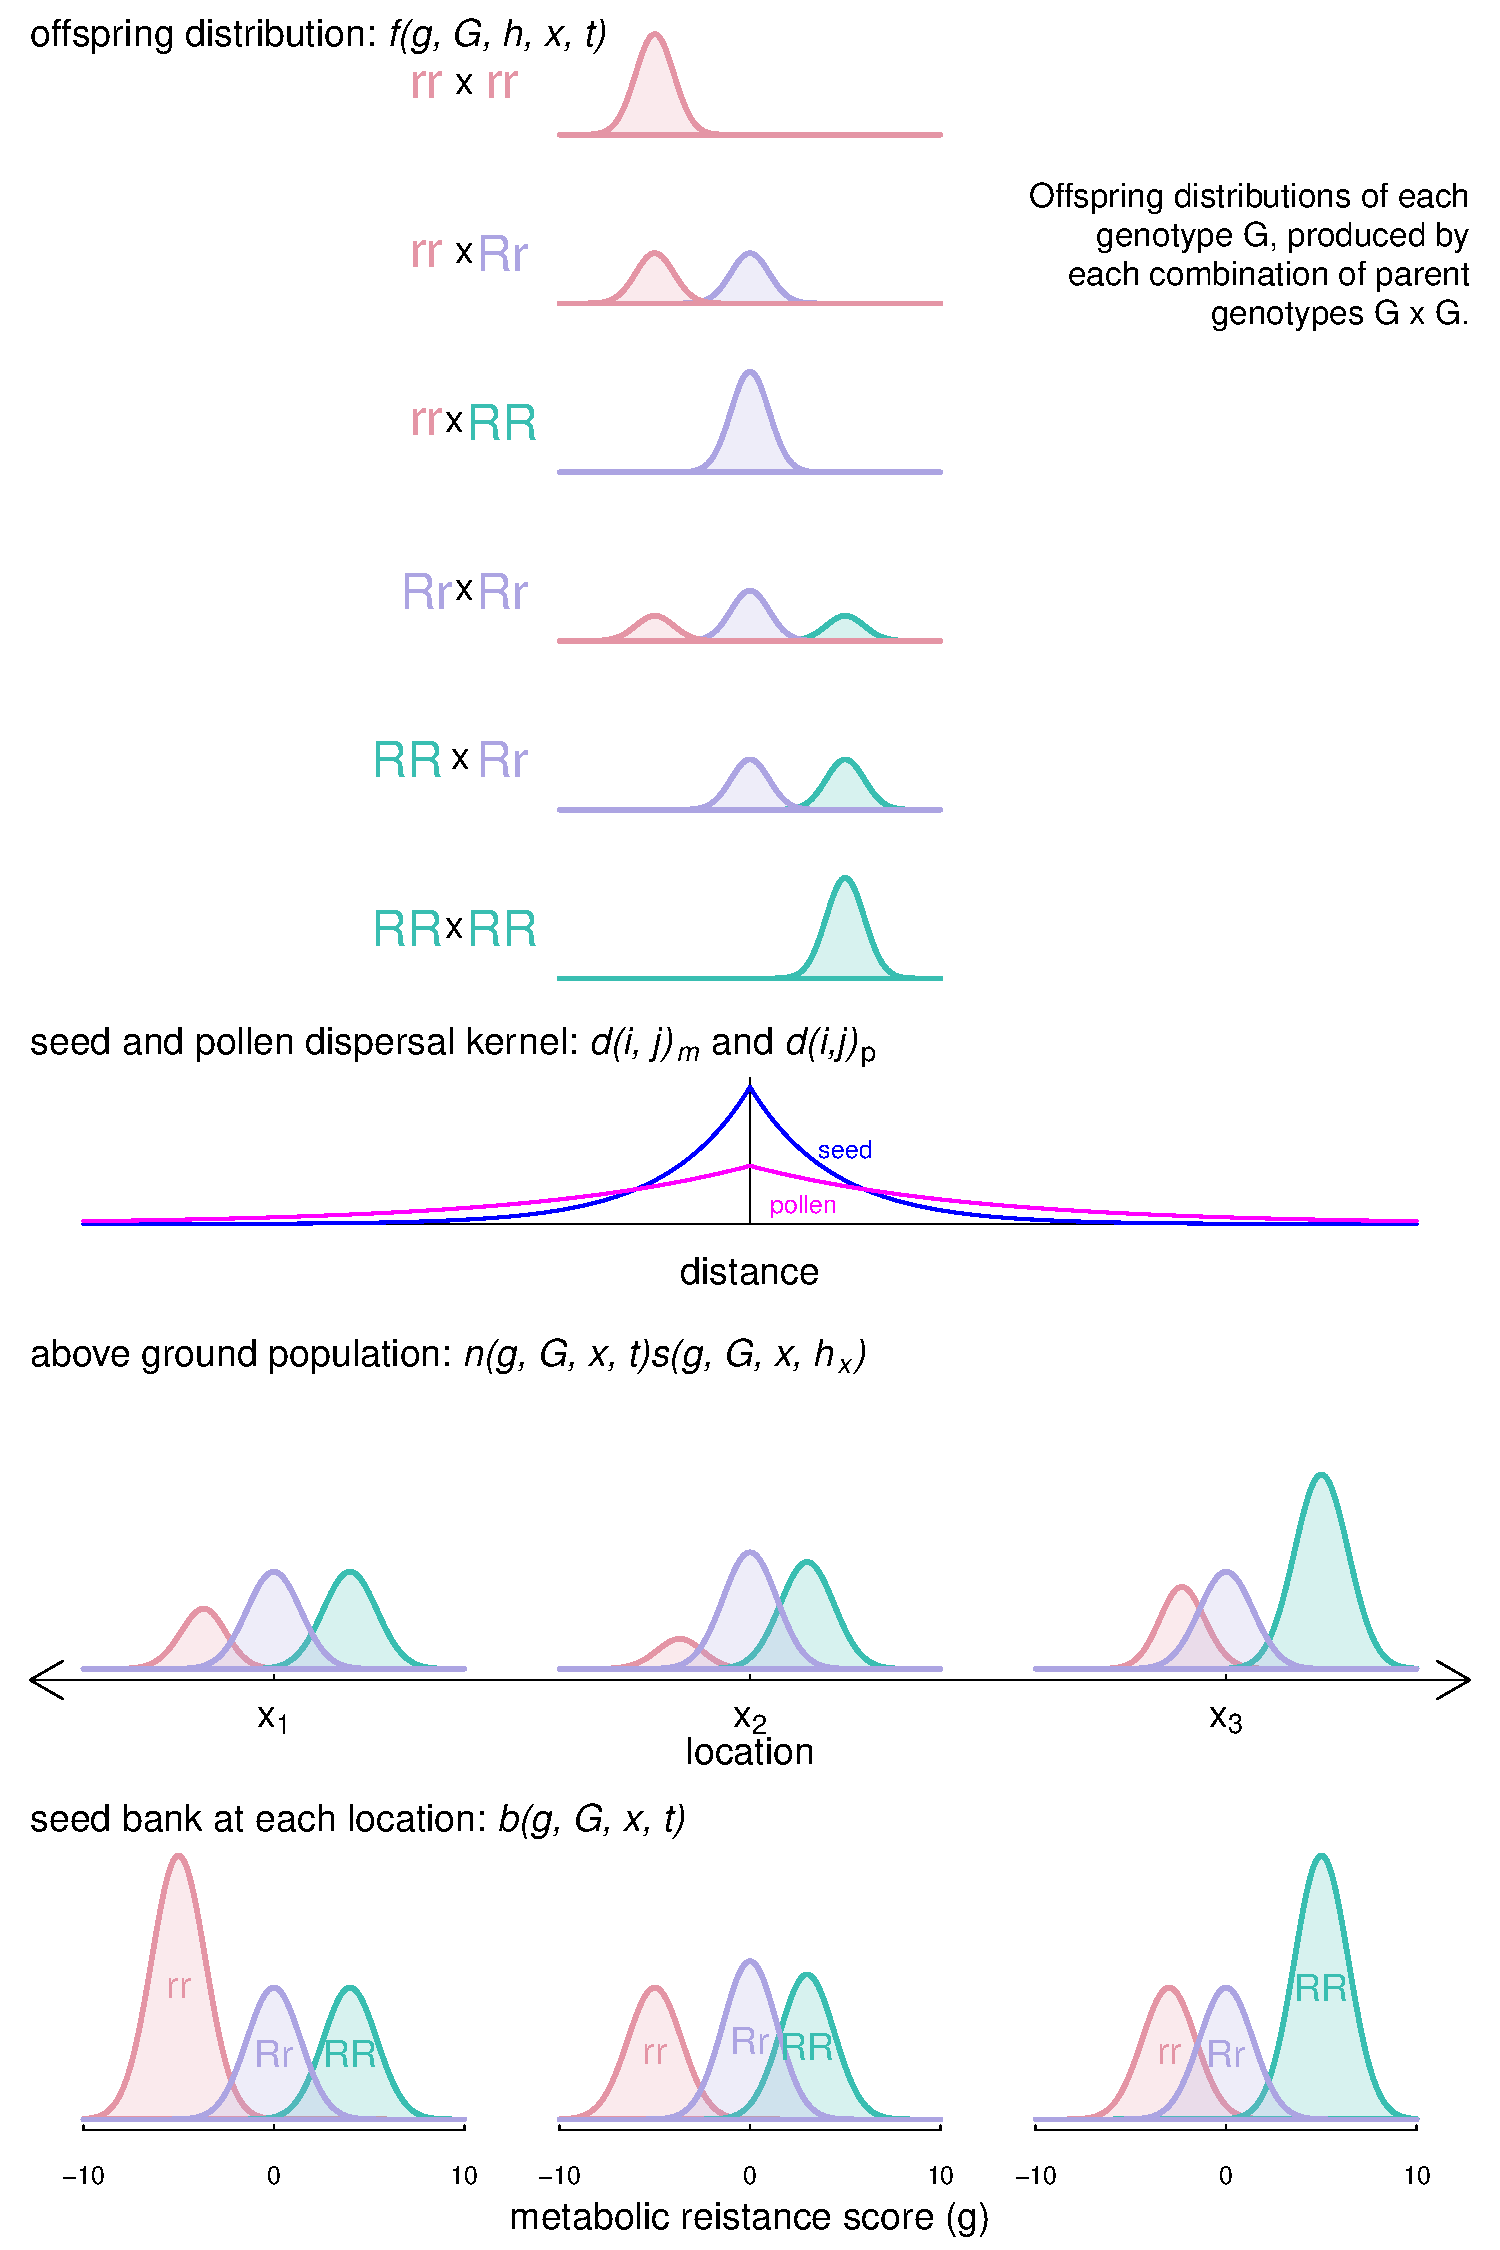
\includegraphics[height=150mm]{/home/shauncoutts/Dropbox/projects/MHR_blackgrass/BG_population_model/writting/figures/spatial_model_fig/BG_pop_spatial_mod_schematic.pdf}
\caption{\bf Schematic of the spatial population model.} At each location $x_i$ seeds in the the seed bank have one of three target site resistance genotypes $G \in \{RR, Rr, rr\}$ and are distributed over metabolic resistance score $g$. The emergence and survival functions, $n(g, G, x, t)s(g, G, x, h_x)$ are applied to the seed bank distributions to get the above ground parent distributions. Those parent distributions are mixed across genotypes (via the target site and quantitative mixing kernels) and locations (via the pollen dispersal kernel) to create the offspring distributions. Seeds are then dispersed between locations using the seed dispersal kernel.
\label{fig:schematic}
\end{figure}

% Place figure captions after the first paragraph in which they are cited.
%\begin{figure}[!h]
%\caption{{\bf Bold the figure title.}
%Figure caption text here, please use this space for the figure panel descriptions instead of using subfigure commands. A: Lorem ipsum dolor sit amet. B: Consectetur adipiscing elit.}
%\label{fig1}
%\end{figure}

The target site mixing function
\begin{subequations}
\begin{equation}\label{eq:TSR_mixing_kern}
	Q(G, G_m, G_p) = \frac{\sum_{\forall k \in G_m \times G_p} q(G, k)}{card\left( G_m \times G_p \right)}
\end{equation}      
\begin{equation}\label{eq:allel_count}
	q(G, k) = \begin{cases}
		1 &\text{if } a_1 \in k \bigwedge a_2 \in k\\
		0 &\text{otherwise} 
	\end{cases}, \text{where } G = \{a_1, a_2\}
\end{equation} 
\end{subequations}
returns the fraction of seeds produced of target site genotype $G$ by parents of target site genotype $G_m$ and $G_p$. Each target site genotype is a set of two alleles, $G = \{a_1, a_2\}$, with $a_i \in \{R, r \}$. The set of all ordered pairs of alleles (i.e. target site genotypes) that can be produced by the parent genotypes is given by the Cartesian product $G_m \times G_p$. $q(G, k)$ is a function that returns one if both alleles of the genotype of interest, $G$, are in proposed ordered pair $k$. To make $Q(G, G_m, G_p)$ a proportion we divide by the cardinality of the Cartesian product, $card \left( G_m \times G_p \right)$. For a fuller explanation, including a brief summary of concepts from set theory and a worked example, see \nameref{S1_Appendix}.

The distribution of quantitative trait $g$ in the offspring of each combination of parental genotypes $G_m$ and $G_p$, at each location $x$ is produced by the double integration in Eq. \ref{eq:fecund}; taken over every combination of metabolic resistance score from the maternal parent distribution, $g_m$, and paternal distribution, $g_p$. The offspring produced by every pair of $g_m$:$g_p$ values are assumed to be normally distributed over $g$ with a mean of $0.5g_m + 0.5g_p$ and a standard deviation of $\sigma_f$ ($\text{N}(\cdot)$ in Eq. \ref{eq:fecund}). The parent distribution for each target site genotype $G$ at location $x$ is $n(g, G, x, t)s(g, G, x, t)$, where 
\begin{equation}\label{eq:above_ground}
	n(g, G, x, t) = b(g, G, x, t)\phi_e\phi_b
\end{equation}
is the number of individuals of target site genotype $G$ that emerge from the seed bank and establish. Note that because $b(g, G, x, t)$ is a distribution so is $n(g, G, x, t)$. The distribution of these emerged individuals that survive, $s(g, G, x, h_x)$, is based in their target site genotype, $G$, their quantitative resistance score, $g$, their location $x$, and whether or not herbicide is applied at location $x$, $h_x \in \{0, 1\}$.   
\begin{equation}\label{eq:sur_G}
	s(g, G, x, h_x) = \begin{cases} 
		\frac{1}{1 + e^{-s_0}} &\text{~if~} G \in G^* \\
		\frac{(1 - \varsigma)}{1 + e^{-s_0}} + \frac{\varsigma}{1 + e^{-\left(s_0^x - h_x\left(\xi - \textbf{min}(\xi, \rho g) \right)\right)}} &\text{~otherwise~} 		
	\end{cases} 
\end{equation}
We assume that seeds which germinate but die before seed set from non-management causes are subsumed into the seed survival term, $\phi_b$. We also assume that any reduction in survival due to increased density is subsumed into the affect of density on fecundity (Eq. \ref{eq:seed_production}). Individuals that emerge later in growing season may not be exposed to herbicide, and $\varsigma$ is the proportion of individuals exposed to the herbicide. Target site resistant individuals are assumed to be completely protected from the effects of the herbicide. $G^*$ is the sub-set of genotypes that give target site resistance. We assume target site resistance is dominant \cite{Neve2007}, thus $G^* \in \{\{R, R\}, \{R, r\}\}$. $s_0$ is the survival probability (in logits) when there is no herbicide, or for individuals not affected by herbicide, for individuals with resistance score $g = 0$. Notice that when $h_x = 0$ the top and bottom condition of Eq. \ref{eq:sur_G} are the same. $\xi$ is the reduction in survival (in logits) caused by herbicide for individuals with a resistance score $g = 0$ and $\rho$ is the protective effect of a one unit increase in resistance score $g$. Because $\rho$ is only meaningful in relation to $\xi$, and $\xi$ is only meaningful relative to $s_0$, we fix $s_0 = 10$ and use $\rho$ and $\xi$ to control the shape of the survival function. 

The number of seeds produced per individual at location $x$, $\psi(g, x)$, is a function of resistance and the density of surviving plants, with greater resistance and higher density reducing the number of seeds. 
\begin{subequations}
\begin{equation}\label{eq:seed_production}
	\psi(g, x) = \frac{\frac{1}{3}f_\text{max}}{1 + \Psi(g) + f_d M(h_x, x, t) + f_dM(h_x, x, t) \Psi(g)}
\end{equation}  
\begin{equation}
	\Psi(g) = 1 + e^{-(f_0 - f_r|g|)}
\end{equation}
\end{subequations}
where $f_\text{max}$ is the maximum possible number of seeds per individual, $f_0$ controls the number of seeds produced when $g = 0$, $|g|$ is the absolute value of $g$, $f_r$ is the cost of resistance in terms of reduction in seed production, $1/f_d$ is the population level where individuals start to interfere with each other and 
\begin{equation}\label{eq:num_sur}
   M(h_x, x, t) = \sum_{\forall G} \int_g n(g, G, x, t)s(g, G, x, h_x)\text{d}g
\end{equation}
is the number of above ground individuals that survive until seed set at location $x$. Because total population is calculates at each location independently we are implicitly assuming that only plants very close to each other affect fecundity (i.e. only plants within $\text{d}x / 2$ of location $x$). The number of seeds produced per individual is reduced by $1/3$ because $\sum_{\forall G_m}\sum_{\forall G_p} Q(G, G_m, G_p) = 3$ in Eq. \ref{eq:fecund}, inflating the total number of new seeds by 3 in Eq. \ref{eq:fecund}.    

Finally both target site and quantitative resistance genes are mixed spatially via the pollen dispersal kernel and the seed dispersal kernel. Spatial mixing requires double integration over the location of the mother, $x_m$, and father, $x_p$ in Eq. \ref{eq:fecund}. The integration over spatial locations takes every pair of locations $x_m:x_p$ and generates a distribution of seeds over metabolic resistance score $g$ for every genotype $G$ at maternal location $x_m$. The distribution of seeds produced is based on the distribution over $g$ of surviving above ground individuals at $x_m$, and the frequency of pollen arriving at site $x_m$ with the genotype $g_p$ and $G_p$. This frequency is calculated as
\begin{equation}\label{eq:pollen_func}
\gamma(g_p, G_p, x_p, x_m, h_x, t) = \frac{n(g_p, G_p, x_p, t)
s(g_p, G_p, x_p, h_x) d_p(x_p, x_m)} {\sum_{\forall G}\int_{x}\int_{g} n(g, G, x, t) s(g, G, x, h_x) d_p(x, x_m) \text{d}g\text{d}x}, 
\end{equation}
where $n(g, G, x, t)$ and $s(g, G, x, h_x)$ are defined in Eq.'s \ref{eq:above_ground} and \ref{eq:sur_G} respectively, and 
\begin{equation}\label{eq:pollen_disp}
	d_p(i, j) = \frac{c}{a^{2/c}\Gamma\left(\dfrac{2}{c} \right)\Gamma\left(1 - \dfrac{2}{c} \right)}{\left( 1 + \dfrac{\delta_{i,j}^c}{a} \right)}^{-1} 
\end{equation} 
is the pollen dispersal kernel. We used a logistic kernel, which was found to be the one of the best fitting pollen dispersal kernels for oil seed rape \cite{Klei2006}. This is a two parameter kernel with a scale, $a$, and shape, $c$, parameter, where $\delta_{i,j}$ is the distance between locations $i$ and $j$. 

The probability that a seed produced at maternal location $x_m$ is dispersed to location $x'$ is 
\begin{subequations}\label{eq:seed_disp}
\begin{equation}\label{eq:seed_kern}
	d_m(i, j) = {\alpha \Upsilon_1 \Omega_1 \delta_{ij}}^{\Omega_1 - 2} e^{-\Upsilon_1 \delta_{ij}^{\Omega_1}} + {(1 - \alpha) \Upsilon_2 \Omega_2 \delta_{ij}}^{\Omega_2 - 2} e^{-\Upsilon_2 \delta_{ij}^{\Omega_2}}  
\end{equation}
\begin{equation}\label{eq:shape}
	\Omega_k = \frac{1}{1 + \text{ln}(1 - \omega_k)}
\end{equation}
\begin{equation}\label{eq:scale}
	\Upsilon_k = \frac{\Omega_k - 1}{{\Omega_k \mu_k}^{\Omega_k}}
\end{equation}
\end{subequations} 
This double Weibull dispersal kernel was found to be the best fit to \textit{A. myosuroides} seed dispersal in a majority of cases \cite{Colb2001}. $\delta_{ij}$ is the distance between locations $i$ and $j$, $\alpha$ is the proportion of seeds in the short dispersal kernel rather than the long dispersal kernel, $\mu_k$ is the distance most seeds disperse to under kernel $k \in \{1, 2\}$. The skew of kernel $k$ is controlled by $\omega_k$, the proportion of seeds that disperse up to distance $\mu_k$. This kernel ignores dispersal by farm machinery \cite{Colb2001}.

The model was implemented in Julia version 0.5.0, and code for the model and plotting is available in \nameref{S1_File}.     

\subsection*{Parametrization}
Several of the population model parameters, particularly those relating to the quantitative genetic selection model, are unknown for our study system. However, we do have field observations with estimates of above ground plant densities and susceptibility to herbicide. While we cannot directly parametrize the model with this data, perform a basic sanity check and use this data to constrain the parameter space to regions that produce sensible results. We outline this procedure in \nameref{S2_Appendix}.  

For this approach to work well we need to constrain the parameter space as much as possible \textit{a prior}. Estimates and sources for each parameter are given in Table \ref{tab:parameters}.          

\begin{table}[!ht]
\begin{adjustwidth}{-2.25in}{0in} % Comment out/remove adjustwidth environment if table fits in text column.
\centering
\caption{
{\bf Model parameters with range used in parameter filtering (see \nameref{S2_Appendix}), etimated value, brief description and source}}
\begin{tabular}{|l+l|l|p{9.5cm}|p{2.5cm}|}
\hline
		{\bf parameter} & {\bf range} & {\bf estimate} & {\bf description} & {\bf source}\\
 \thickhline
 &\multicolumn{4}{l|}{{\it Population model}}\\ \hline
	$\phi_b$ & 0.22 -- 0.79 & 0.42 & seed survival probability & \cite{Thom1997}\\ \hline
	$\phi_e$ & 0.45 -- 0.6 & 0.52 & germination probability & \cite{Colb2006}\\ \hline	
	$f_\text{max}$ & 30 -- 300$^\blacklozenge$ & 45 & seed production (in seeds/plant) of highly susceptible individuals at low densities & \cite{Doyl1986}\\ \hline
	$f_d$ & 0 -- 0.15$^\dag$ & 0.004 & reciprocal of population (1/pop.) at which individuals interfere with each others fecundity & \cite{Doyl1986}\\ \hline 
	$f_0$ & 5 -- 10$^\dag$ & no est$^\ddag$  & fecundity in a naive population in logit($f_0$)$f_\text{max}$ & simulation\\ \hline
	$f_r$ & $0.1f_0$ -- $2f_0 ^\dag$ & no est$^\ddag$ & reduction in fecundity (in logits) due to a one unit increase in resistance. Only meaningful in relation to $f_0$ & simulation\\ \hline
	$\sigma_f$ & fixed & 1 & standard deviation of offspring distribution & fixed without loss of generality\\ \hline
	$s_0$ & fixed & 10 & survival in a naive population is logit($s_0$) & fixed, use $\xi$ and $\rho$ to control survival function\\ \hline
	&\multicolumn{4}{l|}{{\it Management effects}}\\ \hline
	$\varsigma$ & 0.5 -- 1$^\dag$ & 0.8$^\blacklozenge$ & proportion of above ground individuals exposed to herbicide & HGCA\\ \hline   		
	$\xi$ & $2s_0$ -- $3s_0^\dag$ & no est$^\ddag$ & reduction in survival (in logits) due to herbicide (only meaningful in relation to $s_0$) & simulation\\ \hline	
	$\rho$ & $0.1\xi$ -- $2\xi$ & no est$^\ddag$ & protection against herbicide (in logits) conferred by a one unit increase in $g$, only meaningful in relation to $\xi$ & simulation\\ \hline
	int$_{Rr}$ & 0.001 -- 0.2 & & initial frequency of resistant target site genotype. All other individuals are assumed to be of genotype rr & \\ \hline
	&\multicolumn{4}{l|}{{\it Dispersal}}\\ \hline
	$\alpha$ & 0.38 -- 0.58$^\dag$ & 0.48 & proportion of seeds in short dispersal kernel & \cite{Colb2001}\\ \hline   
	$\mu_1$ & 0.46 -- 0.7$^\dag$ & 0.58 & distance (in m) at which maximum number of seeds are found in short seed dispersal kernel & \cite{Colb2001}\\ \hline
	$\mu_2$ & 1.32 -- 1.98$^\dag$ & 1.65 & distance (in m) at which maximum number of seeds are found in long seed dispersal kernel & \cite{Colb2001}\\ \hline
	$\omega_1$ & 0.35 -- 0.53$^\dag$ & 0.44 & proportion of seeds that disperse up to distance $\mu_1$ in short seed dispersal kernel & \cite{Colb2001}\\ \hline
	$\omega_2$ & 0.31 -- 0.47$^\dag$ & 0.39 & proportion of seeds that disperse up to distance $\mu_2$ in long seed dispersal kernel & \cite{Colb2001}\\ \hline
	$a$ & 25.6 --38.4$^\dag$ & 32.3 & scale parameter for pollen dispersal kernel & \cite{Klei2006}\\ \hline
	$c$ & 2.66 -- 3.98$^\dag$ & 3.32 & shape parameter for pollen dispersal kernel & \cite{Klei2006}\\ \hline
\end{tabular}
\begin{flushleft} $\blacklozenge$ sourced from grey literature, unpublished data and expert opinion\\
	$\dag$ range not available from literature, simulation used to find plausible range\\
	$\ddag$ no estimate not available from literature, simulation used to find plausible range
\end{flushleft}
\label{tab:parameters}
\end{adjustwidth}
\end{table}

\subsection*{Sensitivity analysis}
The sanity check resulted in 11,866 parameter combinations that produced black grass populations which fell in the acceptable range. We performed a global sensitivity analysis on this set of 11,866 parameter sets to explore how different parameters, and their interactions, affected the behaviour of the model. We followed the approach of \cite{Cout2014} and fit Boosted Regression Trees (BRTs) to find relationships between the parameter values and the model behaviours of interest. We are primarily interested in three aspects of the models behaviour; the speed at which target site resistance establishes in the population, the importance of quantitative resistance, and how fast the population overall spread. We used the proportion of alleles that are $R$ in the final time step as a metric of target site resistance spread, the survival of target site susceptible individuals under herbicide at the maximum $g$ achieved as a metric of how important quantitative resistance was, and mean spread rate as a metric of population spread. For a detailed explanation of the sensitivity analysis see \nameref{S2_Appendix}.

\subsection*{Simulation experiments}
Our aim is to generate hypotheses about how the initial conditions of the invasion of a new resistance genotype (defined by both $G$ and $g$) can change how that invasion develops over time. Our model assumes no mutations in the target site resistance loci. For target site resistance to develop in a population the target site resistant allele needs to be introduced from a population where it has already developed through mutation. It is also possible to import high levels of quantitative resistance. To explore how the introduction context affects the evolution of resistance we created two general scenarios: the transplant scenario (Fig. \ref{fig:exper}A) where a small number of seeds are deposited in the center of a receiving landscape; and a natural spread scenario, where target site resistance starts at one edge of the landscape, and is allowed to invade into rest of the landscape (Fig. \ref{fig:exper}B). The transplant scenario replicates the situation when a small amount of seeds are transported to a new, distant, area by farm vehicles. The natural spread scenario replicates spread at a smaller scale, where the target site genotype is invading into a neighbouring field (possibly under different management), or from a field margin. The different characteristics of the source and receiving populations replicate populations with different management histories, and those that are under different selection pressures.     

\newpage
\begin{figure}[!h] 
	\includegraphics[height=100mm]{/home/shauncoutts/Dropbox/projects/MHR_blackgrass/BG_population_model/writting/figures/experiments_schematic.pdf}
\caption{\bf Schematic of simulation experiments.} {\bf A)} Transplant experiments where 10 seeds are added to the seed bank at the center of the receiving landscape after 20 time steps. The added seeds have one of four combinations of frequency of target site resistance and the amount of quantitative resistance representing real world situations (coloured text in source population plane). The receiving population was in one of three states (empty, exposed to herbicide for 20 time steps, naive to herbicide). After the 20 time step establishment period the entire landscape was exposed to herbicide. {\bf B)} Natural spread experiments where the source and receiving populations exist on the same landscape. Source populations started with 1\% of alleles being target site resistant (i.e. $R$), while receiving populations started with no target site resistance. In locations exposed to herbicide it is applied continuously for 150 time steps. In both transplant and natural spread experiments non-empty locations were initialized with 10 $rr$ individuals, with low quantitative resistance ($g = 0$). 
\label{fig:exper}
\end{figure}

% Results and Discussion can be combined.
\section*{Results}
The ecological and genetic background against which the invasion of the resistance genotype took place had an enormous effect on how the two genetic architectures underlying resistance (target site and quantitative resistance) interacted. In both the transplant and natural spread experiments it was only when populations with small amounts of target site resistance expanded into empty landscapes that target site resistance became the dominant mode of resistance. The details of how this develops over time are best shown by examining a run of the natural spread experiment (Fig. \ref{fig:pro_R_natspr}). When the larger part of the landscape (the receiving area in Fig. \ref{fig:pro_R_natspr}) is exposed to herbicide, and the invasion is into an empty landscape (Fig. \ref{fig:pro_R_natspr}a,b), the target site resistance allele quickly becomes prevalent in the population. This occurred because under these conditions the target site resistance allele developed in the population early, before it has completely invaded into the empty area (white regions on the left hand side of the heat maps). After target site resistance had become established in the population it spread with the population and so became established over the whole landscape. Even when the source region was not exposed to herbicides, target site resistance alleles eventually invaded back into source population, leading to high levels of target site alleles in the part of the landscape that was not exposed to herbicide. When only the smaller source region is exposed to herbicide there is not enough selective pressure to drive the target site resistance allele into the unexposed area, although seed and pollen imports from the source region mean that approximately 10\% of target site alleles are resistant in the naive area (Fig. \ref{fig:pro_R_natspr}c).            

\begin{figure}[!h] 
	\includegraphics[height=80mm]{/home/shauncoutts/Dropbox/projects/MHR_blackgrass/BG_population_model/model_output/pro_R_time_space.pdf}
\caption{\bf Invasion of target site resistant allele, $R$, in the natural spread experiments.} The population over the whole landscape (y-axis) is shown at each time step (x-axis; i.e. each slice is a snapshot of the population).  Colour intensity shows population density at each location at each time step, with empty locations being white. Hue indicates the proportion of all alleles at a location and time that are $R$, with high values (reds) indicating that almost all resistance to herbicide is due to target site resistance. In a), b) and c) the source population (containing target site alleles) is invading into an empty landscape, while in d), e) and f) the source population is invading into an area that already has \textit{A. myosuroides} present, but no target site resistance alleles. Each column shows a different pattern of herbicide application. We do not show the combination where both source and receiving populations are naive to herbicide as there is no selective pressure, and so development of resistance under this herbicide regime.    
\label{fig:pro_R_natspr}
\end{figure}

The dynamics of the system are very different when the target site alleles are invading into an area that already has \textit{A. myosuroides}. In these cases target site alleles invade very slowly (reds and purples stay near the source region in Fig. \ref{fig:pro_R_natspr}d,f). When the receiving region was exposed to herbicide the population already there developed high levels of quantitative resistance by the time the target site resistant alleles reached that part of the landscape (\nameref{S1_Fig}). These high levels of metabolic resistance reduced the survival difference between target site resistant and target site susceptible individuals, reducing the selective pressure and slowing the spread of target site resistant alleles. This result is some what surprising since the pollen dispersal kernel is quiet flat at the scales examined in these experiments, and so target site resistant alleles could reach large parts of the receiving landscape. Target site alleles did still spread through landscapes with high levels of quantitative resistance due to the higher demographic costs of quantitative resistance, but at a much slower rate.    

Populations only displayed both high levels of quantitative resistance and high frequencies of target site resistance alleles when herbicide was applied to the receiving population, and when the target site resistance alleles were invading in to a region that already had \textit{A. myosuroides} (Fig. \ref{fig:both_natspr}d,e). Even then both genetic architectures were only important at the invasion front of the target site resistant alleles(purple region in Fig. \ref{fig:both_natspr}d,e). This occurred because the target site resistant alleles could only invade slowly into the receiving region. This allowed time for levels of quantitative resistance to build up, and these high quantitative resistance genes were then imported back into the region, with high target site resistance, increasing quantitative resistance there.        

\begin{figure}[!h] 
	\includegraphics[height=80mm]{/home/shauncoutts/Dropbox/projects/MHR_blackgrass/BG_population_model/model_output/sur_rr_and_proR_time_space.pdf}
\caption{\bf regions and times where both high frequencies of the target site resistant allele, $R$ and high quantitative resistance occurred in the natural spread experiments.} The population over the whole landscape (y-axis) is shown at each time step (x-axis; i.e. each slice is a snapshot of the population).  Colour intensity shows population density at each location at each time step, with empty locations being white. Hue indicates the proportion of all alleles at a location and time that are $R$, multiplied by the survival of target site susceptible individuals under herbicide. In a), b) and c) the source population (containing target site alleles) is invading into an empty landscape, while in d), e) and f) the source population is invading into an area that already has \textit{A. myosuroides} present, but no target site resistance alleles. Each column shows a different pattern of herbicide application. We do not show the combination where both source and receiving populations are naive to herbicide as there is no selective pressure, and so development of resistance under this herbicide regime.    
\label{fig:both_natspr}
\end{figure}

In our model target site resistant individuals are, by definition, fitter than target site susceptible individuals under herbicide application. Target site resistant individuals have higher survival, and do not have to incur the demographic costs of high quantitative resistance. However, the demographic costs of quantitative resistance ($f_r$) are incurred whether and individual is using quantitative resistance or not. As a result the fitness difference between target site resistant individuals and target site susceptible individuals can be small to moderate in parts of the landscape where target site resistant individuals are rare (\nameref{S2_Fig}). This occurs because high levels of quantitative resistance build up in these regions, and so genotypes with high levels of quantitative resistance are very prevalent in the pollen. This swamps the pollen from the target site resistant individuals and means that their offspring also tend to have high levels of quantitative resistance. Even if that trait is not useful for them, they still incur much of the demographic cost.

The sensitivity analysis showed that the protective effect of a one unit increase in the quantitative resistance trait $g$ ($\rho$) and the demographic costs of quantitative resistance ($f_f$), had the largest effect on genetic dynamics of the population (\nameref{S2_Appendix}). These parameters are crucially important for when both genetic architectures can co-exist, with co-existence only common at $f_r < 0.8$ and $\rho > 1.25$ and being more common when the  population was invading into and empty landscape (\nameref{S3_Fig}c,d)   

We use transplant experiments to model situations where genes from populations with different management histories, and thus different levels of target site and quantitative resistance, invade into a new population. A situation commonly arising with long distance dispersal of propagules. These experiments show that the characteristics of the source population and receiving area, and the protective effect of quantitative resistance, $\rho$, all influence the simultaneous evolution of both target site and quantitative resistance. 

Regardless of the genetic structure of the introduced seeds, if those seeds were introduced into a landscape where \textit{A. myosuroides} was already present (light and dark blue lines in Fig. \ref{fig:transloc_gpro}) target site and quantitative resistance could only co-exist over a small range of values for $\rho$. Either target site resistance dominated (solid blue lines high and dashed blue lines low) or quantitative resistance dominated (dashed blue lines high, solid blue lines low). This pattern was most pronounced when the receiving population (where target site resistance was absent) had been exposed to herbicide before target site alleles were introduced (dark blue lines). When the receiving population was naive to herbicide (light blue lines) the level of quantitative resistance in the population after 100 years still showed a threshold relationship with $\rho$, but amount target site resistance in the population reduced more slowly with increasing $\rho$. Thus, target site and quantitative resistance co-existed over a greater range of values when target site alleles were introduced to a naive population.

When target site resistant alleles were introduced into an empty landscape the genotype of the source population had a large effect on how the invasion unfolded. When the source population had low quantitative resistance and a low frequency of target site resistance alleles target site resistance was always high, and quantitative resistance also became important at high values of $\rho$ (black lines Fig. \ref{fig:transloc_gpro}a). When the source populations had a high frequency of target site resistant alleles and low quantitative resistance target site resistance always dominated (black lines Fig. \ref{fig:transloc_gpro}b). When the source population had low target site resistance and high quantitative resistance, both genetic architectures could co-exist in the population, over a wide range of values for $\rho$, although at very low values of $\rho$ target site resistance dominated, and at very high values of $\rho$ quantitative resistance dominated (black lines Fig. \ref{fig:transloc_gpro}c). When the source population had both high quantitative resistance and high target site resistance, then target site resistant alleles were very preventible in the population for all the values of $\rho$ we tested. At values of $\rho > 1$ the population also had high levels of quantitative resistance (Fig. \ref{fig:transloc_gpro}d).                      

\begin{figure}[!h] 
	\includegraphics[height=90mm]{/home/shauncoutts/Dropbox/projects/MHR_blackgrass/BG_population_model/model_output/effect_g_pro_resist.pdf}
\caption{\bf Effect of $\rho$ (protective effect of $g$) on target site and quantitative resistance in transplant experiments.} All populations had a establishment period of 20 time steps and were then exposed to herbicide for 100 time steps, after which time target site and quantitative resistance were measured. Target site resistance was measured as percentage of all alleles in the population that are $R$ (solid lines). Quantitative resistance was measured as the survival of target site susceptible individuals ($rr$) under herbicide application (dashed lines). We tested source populations with four different combinations of target site and quantitative resistance (a, b, c, d), and three different types of receiving landscape: empty--black lines, \textit{A. myosuroides} already present and naive to herbicide--light blue lines, and \textit{A. myosuroides} already present and exposed to herbicide for 20 time steps--dark blue lines.        
\label{fig:transloc_gpro}
\end{figure}

\section*{Discussion}
We find that the ecological and historical context surrounding the invasion of target site resistance into a new area can have an enormous effect on how that invasion unfolds and which genetic architecture dominates. The invasion of target site resistance alleles was much slower when the invasion was into an area that already contained \textit{A. myosuroides}. In addition the frequency of target site resistance and amount of quantitative resistance changed very quickly over space, and on the target site resistance invasion front both architectures co-existed for long periods of time. This occurred even though target site resistance conferred perfect resistance with no demographic costs, giving target site resistant individuals a competitive advantage over those individuals with only quantitative resistance. When the invasion occurred into an empty landscape its dynamics were determined the genetic architecture of the source population. Depending on the architecture of the source population all resistance in a population could be target site, it could be target site or quantitative depending on how effective quantitative resistance was, or high levels of both target site and quantitative resistance could coexist. Given this variability we might expect to see different architectures predominate in different regions of a landscape. To date there is little evidence to either support or refute this hypothesis because the prevalence and type of resistance has not typically been studied at landscape scales [SOME REVIEW REF].

Co-existence of both target site and quantitative resistance occurred across the whole population when the invasion occurred into an empty landscape. This suggests that co-existence will be most common at the leading edge of an invasion, where expanding nascent population foci are common \cite{Mooy1988}.

From a management perspective target site and quantitative resistance mean different things. Target site resistance typically provides very high levels of protection from the poison and incurs few demographic costs \cite{Bauc2016}. This means that once it is established in a population it will be present in the genome over the long term, even after the poison is no longer used [REF]. However, target site resistance often only protects against a single chemical family, and so strategies like compound cycling can delay the evolution of target site resistance \cite{Rex2013}. The continuous nature of quantitative resistance means that there is always some variation for selection to act on, and it does not rely on de novo mutation or gene importation, and so it can build up earlier. Quantitative resistance uses more general mechanisms such as metabolizing the poison and transporting it, and so can also give cross resistance between compounds \cite{Bauc2016, Neve2007}. On the other hand, it provides less protection from the poison and does incur some (although often small) demographic costs \cite{Bauc2016}. Places where both architectures co-exist may experience the worst of both worlds, resistance that develops very quickly, with very high levels of resistance to existing compounds \cite{Vera2015}, and cross resistance to novel compounds when they are introduced \cite{Neve2007}.   
                         
Because we assume target site resistance is both more effective and less costly than quantitative resistance, under constant selection all resistance in the population will eventually be target site resistance. However, quantitative resistance can occur for long periods of time when it has a low demographic cost, and has a strong protective effect. In our model these quantities were fixed parameters. In reality both the protective effect of quantitative resistance, and the demographic costs it incurs will also be under selection. Over time the metabolic pathways and other mechanisms of quantitative resistance that provide the most protection for the least demographic cost, will predominate. This gives reason to believe that quantitative resistance can be highly effective and have a low demographic costs.    

\section*{Conclusion}
Resistance affects food production systems and human health across the global. Our results suggest that quantitative resistance can greatly slow the invasion of target site resistance, and the evolutionary dynamics within nascent population foci on the invasion front can result in a different genetic architectures dominating or co-existing. As a result we should expect the genetic architecture underlying resistance to be heterogeneous at both local and landscape scales. It follows from this that the effectiveness of different resistance management strategies, like compound cycling and very high doses, may also vary over space, as these different strategies exploit weaknesses in different genetic architectures \cite{Rex2013}. Our model is a first step in generating hypothesis on how the different genetic architectures that underlie resistance will interact across space. It is imperative that this work is followed by empirical observations and experimental tests. A logical starting point would be spatially extensive surveys of resistant populations to see where and when target site and quantitative resistance dominate or co-exist.

\section*{Supporting Information}

% Include only the SI item label in the paragraph heading. Use the \nameref{label} command to cite SI items in the text.
\paragraph*{S1 Fig.}
\label{S1_Fig}
{\bf Heat maps of survival of target site susceptible plants under herbicide}, a measure of the importance of quantitative resistance. These plots show the development of quantitative resistance over time and space, under three patterns of herbicide use.

\paragraph*{S2 Fig.}
\label{S2_Fig}
{\bf Relative difference in life time fitness between target site resistant and target site susceptible individuals.} Heat maps (over time and space) of the ratio of target site resistant lifetime fitness to target site susceptible life time fitness. 

\paragraph*{S3 Fig.}
\label{S3_Fig}
{\bf The frequency of target site resistant alleles (\%R) and the amount of target site and quantitative resistance coexistence, over $f_r$ and $\rho$ parameter space.} 

\paragraph*{S1 File.}
\label{S1_File}
{\bf Julia implementation of model and plotting code}  

\paragraph*{S1 Appendix.}
\label{S1_Appendix}
{\bf Target site mixing function.} 
Expanded explanation and worked example of the target site mixing function $Q(G, G_m, G_p)$.

\paragraph*{S1 Appendix.}
\label{S2_Appendix}
{\bf Parameter sanity check and sensitivity analysis} 

\section*{Acknowledgments}
We thank some people for some things

\nolinenumbers

% Either type in your references using
% \begin{thebibliography}{}
% \bibitem{}
% Text
% \end{thebibliography}
%
% or
% % Compile your BiBTeX database using our plos2015.bst
% style file and paste the contents of your .bbl file
% here.
% 
%\begin{thebibliography}{10}
%
%\bibitem{bib1}

%Conant GC, Wolfe KH.
%\newblock {{T}urning a hobby into a job: how duplicated genes find new
%  functions}.
%\newblock Nat Rev Genet. 2008 Dec;9(12):938--950.

%\end{thebibliography}

%REMEMBER TO FIX UP THESE CITATIONS AND USE THEIR FORMATTING ONCE I HAVE A MORE COMPLEATE VERSION.

%\bibliographystyle{/home/shauncoutts/Dropbox/shauns_paper/referencing/bes} 
\bibliography{/home/shauncoutts/Dropbox/shauns_paper/referencing/refs}


\end{document}

